\documentclass[fsharpNotes.tex]{subfiles}
\graphicspath{ {./figures/} }

\begin{document}

\chapter{Lists}
\label{chap:lists}
\abstract{
  In programming, a list is an abstract data type, which contains a list of elements, such as a list of shopping items \Cref{fig:shoppingList}, a list of students in a class, and a to-do list.
    \begin{figure} % We want the figure on the first page with the chapter title
    \centering
    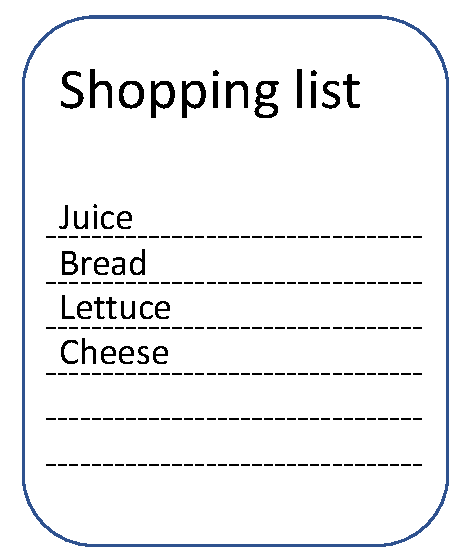
\includegraphics[width=0.5\textwidth]{shoppingList} % for some reason, it does not want to read the pdf-file
    \caption{A list of shopping items.}
    \label{fig:shoppingList}
  \end{figure}
Cornerstones in functional programming are immutable values and functions, and in the previous chapters, we have looked at many ways where this is sufficient for solving many problems. However, often data is on the form of a list in which equivalent expressions need to be calculated and possibly collected into a single value. For example, for the shopping list, we may want to estimate the total shopping price by 1) replacing each item on the list with a price, and 2) summing the elements. In functional programming, this can be done with the programming concept of map and fold, where map produces a new list as the elements of the original list with a function applied to them, and fold sequentially combines the values of the price-list by iteratively adding the price to a subtotal. These are important examples of the usage of lists, but there is more. In this chapter, you will learn how to 
\begin{itemize}
\item define lists
\item manipulate lists using indexing and its properties
\item use the list module including the map and fold higher-order functions.
\end{itemize}
After you have read this chapter, you will be able to model situations such as
\begin{itemize}
\item a class with lists of student records.
\item a drawing consisting of a list of elements, such as a house, some trees, etc.
\end{itemize}
}

\idx[list]{Lists} are unions of immutable values of the same type. A list can be expressed as a \idx{sequence expression},
%
\begin{verbatimwrite}{\ebnf/lists.ebnf}
[[*<*expr*>{*; <*expr*>*}*]]
\end{verbatimwrite}
\syntax{\ebnf/lists.ebnf}{The syntax for a list using the sequence expression.}
%
For example, \mbox{\lstinline![1; 2; 3]!} is a list of integers, \mbox{\lstinline!["This"; "is"; "a"; "list"]!} is a list of strings, \mbox{\lstinline![(fun x -> x); (fun x -> x*x)]!} is a list of functions, and \lstinline![]! is the empty list. Lists may also be given as ranges,
%
\begin{verbatimwrite}{\ebnf/listsRange.ebnf}
[<*expr*> .. <*expr*> [*.. <*expr*>*]]
\end{verbatimwrite}
\syntax{\ebnf/listsRange.ebnf}{The syntax for a list using the range expressions.}
%
where \lstinline[language=syntax]{<*expr*>} in \idx{range expressions} must be of integers, floats, or characters. Examples are \mbox{\lstinline![1 .. 5]!}, \mbox{\lstinline![-3.0 .. 2.0]!}, and \mbox{\lstinline!['a' .. 'z']!}. Range expressions may include a step size, thus, \mbox{\lstinline![1 .. 2 .. 10]!} evaluates to \mbox{\lstinline![1; 3; 5; 7; 9]!}.

F\# implements lists as linked lists, as illustrated in \Cref{fig:linkedList}.
\begin{figure}
  \centering
  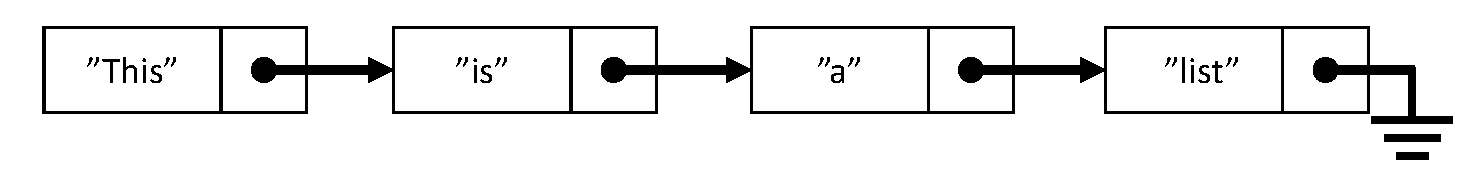
\includegraphics[width=0.95\textwidth]{linkedList}
  \caption{A list is a linked list: Here is illustrated the linked list of \mbox{\lstinline!["This"; "is"; "a"; "list"]!}.}
  \label{fig:linkedList}
\end{figure}
A linked list is a data structure consisting of a number of elements, where each element has an item of data and a pointer to the next element. For lists, every element can only have one other element pointing to it. The first element in a list is called its \idx{head}, and the remainder of the list is called its \idx{tail}. The last element in a list does not point to any other, and this is denoted by the \idx{ground} symbol as shown in the figure. 

A list type is identified with the \idx[list@\keyword{list}]{\keyword{list}} keyword, such that a list of integers has the type \lstinline!int list!. Like strings, lists may be indexed and sliced using the \idx[{[]}@\lstinline{[]}]{\lexeme{[]}} notation, and the first element has index 0, and the last has the one minus the list's length, see \Cref{listIndexing} for examples.
%
\fs{listIndexing}{Lists are indexed as strings and has a \lstinline{Length} property.}
%

A list has a number of \idx[property]{properties}, which is summarized below:
\begin{description}
\item[\texttt{Head}:] Returns the first element of a non-empty list.
  \fsOutputNF{listHeadProp}{\lstinline{Head}}~\\
  Hence, given a non-empty list \lstinline{lst}, then \lstinline{lst.Head = lst[0]}.
  \idxss{Head@\lstinline{Head}}
\item[\texttt{IsEmpty}:] Returns true if the list is empty and false otherwise.
  \fsOutputNF{listIsEmptyProp}{\lstinline{IsEmpty}}~\\
  Hence, given a list \lstinline{lst}, then \lstinline{lst.IsEmpty} is the same as \lstinline{lst = []}.
  \idxss{IsEmpty@\lstinline{IsEmpty}}
\item[\texttt{Length}:] Returns the number of elements in the list.
  \fsOutputNF{listLengthProp}{\lstinline{Length}}~\\
  In contrast to the other properties, there is no equally brief way to express this in F\#.
  \idxss{Length@\lstinline{Length}}
\item[\texttt{Tail}:] Returns the list, except for its first element. The list must be non-empty.
  \fsOutputNF{listTailProp}{\lstinline{Tail}}~\\
  Hence, given a non-empty list \lstinline{lst}, then \lstinline{lst.Tail=lst[1..]}.
  \idxss{Head@\lstinline{Tail}}
\end{description}

\begin{comment}
  Therefore, indexing in lists using \idx{for}-loops is supported using a special notation with the \idx[in@\lstinline{in}]{\keyword{in}} keyword,
\begin{verbatimwrite}{\ebnf/forLoopIn.ebnf}
for <*ident*> in <*list*> do <*bodyExpr*> [*done*]
\end{verbatimwrite}
\syntax{\ebnf/forLoopIn.ebnf}{For-in loop within expression.}
In \keyword{for}-\keyword{in} loops, the loop runs through each element of the \lstinline[language=syntax]{<*list*>}, and assigns it to the identifier \lstinline[language=syntax]{<*ident*>}. This is demonstrated in \Cref{listFor}.
%
\fs{listFor}{The \keyword{for}-\keyword{in} loops are preferred over \keyword{for}-\keyword{to} loops.}
%
Using \keyword{for}-\keyword{in}-expressions remove the risk of off-by-one indexing errors, and thus, \advice{\keyword{for}-\keyword{in} is to be preferred over \keyword{for}-\keyword{to}.}

Lists support slicing identically to strings, as demonstrated in \Cref{listSlicing}.
%
\fsOutput{listSlicing}{Examples of list slicing. Compare with \Cref{stringIndexing}.}
%
\end{comment}

A new list may be generated by concatenated two other lists using \idx[list concatenation]{concatenation} operator, \idx[{@}@{\lstinline{@}}]{\lexeme{@}}.\jon{why does the at-symbol not appear in the index?} Alternatively, a new list may be generated by prepending an element using the \idx[list cons]{cons} operators,  \idx[::@\lstinline{::}]{\lexeme{::}}. This is demonstrated in \Cref{listCon}.
%
\fsOutput{listCon}{Examples of list concatenation.}
%
Since lists are represented as linked lists, the cons operator is very efficient and has computational complexity $\mathcal{O}(1)$, while concatenation has computational complexity $\mathcal{O}(n)$, where $n$ is the length of the first list.

Pattern matching in the \keyword{match}--\keyword{with} expression is possible with combination of the \lexeme{[]} and \lexeme{::} notations in a manner similar to indexing and prepending elements. For example, recursively iterating over list is often done as illustrated in \Cref{listRecursive}.
%
\fs{listRecursive}{Using \keyword{match}--\keyword{with} to recursively print the elements of a list.}
%
The \keyword{match}--\keyword{with} expression recognizes explict naming of elements such as 3-element list \lstinline{[s;t;u]}, and the cons-notation \lstinline{head::tail}, where \lstinline{head} is the first element of a non-empty list, and \lstinline{tail} is the possibly empty tail. In particular, patterns for single element list can either be \lstinline{head::[]}, \lstinline{[head]}, or \lstinline{s when s.Length = 1}.

It is possible to make multidimensional lists as lists of lists, as shown in \Cref{listMultidimensional}. 
%
\fs{listMultidimensional}{A ragged multidimensional list, built as lists of lists, and its indexing.}
%
The example shows a \idx{ragged multidimensional list}, since each row has a different number of elements. This is also illustrated in \Cref{fig:raggedLinkedList}.
\begin{figure}
  \centering
  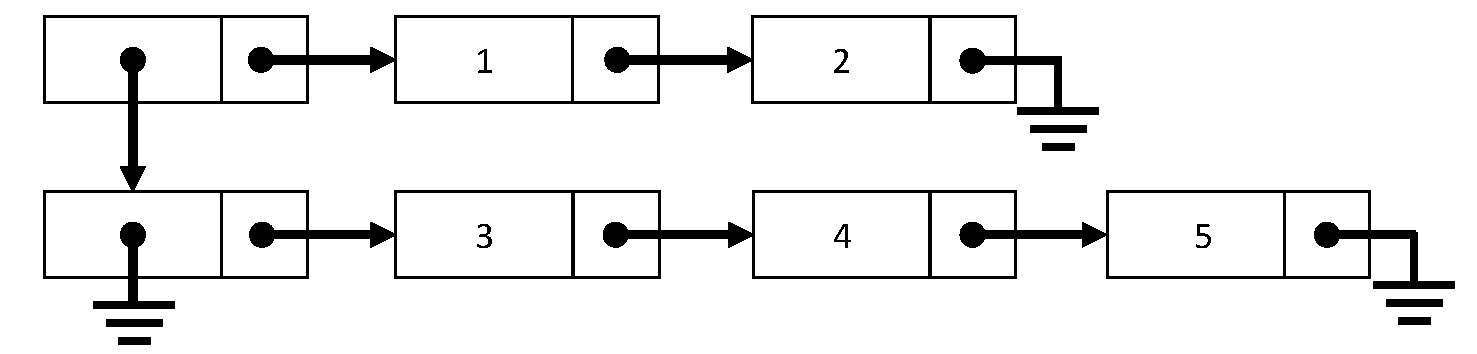
\includegraphics[width=0.9\textwidth]{raggedLinkedList}
  \caption{A list is a ragged linked list: Here is illustrated the linked list of \mbox{\lstinline![[1;2];[3;4;5]]!}.}
  \label{fig:raggedLinkedList}
\end{figure}

Operations on data structures are often analyzed for their \idx{computational complexity}, which is a worst-case and relative measure of their running time on a given piece of hardware. The notation is sometimes called \idx{Big-O} notation or \idx{asymptotic notation}. For example, the algorithm for calculating the length of a linked list starts at the head and follows the links until the end. For a list of length $n$, this takes $n$ steps, and hence the computational complexity $\mathcal{O}(n)$. Technically speaking, if the true running time as a function of the length of the list is $f(n)$, then there exists a positive real number $A$ and a real number $n_0$ such that for all $n\leq n_0$,
\begin{equation}
  |f(n)| \leq Ag(n).
\end{equation}
I.e., if $n$ is large enough, then the running time grows no faster than $Mn$ for some constant $M$. This constant will differ per computer, but the asymptotic notation describes the relative increase in running time as we increase the list size. Similarly, indexing an element $i$ of a list of length $n$ is also $\mathcal{O}(n)$, since in the worst case, $i=n$, and the linked list must be traversed from the head to its tail. This is slow in comparison to arrays, see \Cref{sec:arrays}.
 
\section{The List Module}
Lists are so commonly used that a \idx[list module]{module} is included with F\#. A module is a library of functions and will be discussed in general in \Cref{sec:modules}. The list of functions in the list module is very long, and here, we briefly showcase some important ones. Below, the functions are grouped into 3: Simple functions, which take and/or give lists as argument and/or results; higher-order functions, which takes a function as an argument; and those that mimic the list's properties which can be useful in conjunction with the higher-order functions. Higher-order functions are discussed in detail in \Cref{chap:higherOrderFunctions}.

Some often used simple functions in alphabetical order are:
\begin{description}
%\item[\texttt{List.ofArray}:] \lstinline{arr:'T [] -> 'T list}.~\\
%  Returns a list whose elements are the same as \lstinline{arr}. See \Cref{sec:arrays} for more on arrays.
%  \fsOutputNF{listOfArray}{\lstinline{List.ofArray}}\idxss{List.ofArray@\lstinline{List.ofArray}}
\item[\texttt{List.rev}:] \lstinline{lst:'T list -> 'T list}.~\\
  Returns a new list with the same elements as in \lstinline{lst} but in reversed order.
  \fsOutputNF{listRev}{\lstinline{List.rev}}\idxss{List.rev@\lstinline{List.rev}}
\item[\texttt{List.sort}:] \lstinline{lst:'T list -> 'T list}.~\\
  Returns a new list with the same elements as in \lstinline{lst} but where the elements are sorted.
  \fsOutputNF{listSort}{\lstinline{List.sort}}\idxss{List.sort@\lstinline{List.sort}}
%\item[\texttt{List.toArray}:] \lstinline{lst:'T list -> 'T []}.~\\
%  Returns an array whose elements are the same as \lstinline{lst}.  See \Cref{sec:arrays} for more on arrays.
%  \fsOutputNF{listToArray}{\lstinline{List.toArray}}\idxss{List.toArray@\lstinline{List.toArray}}
\item[\texttt{List.unzip}:] \lstinline{lst:('T1 * 'T2) list -> 'T1 list * 'T2 list}.~\\
  Returns a pair of lists of all the first elements and all the second elements of \lstinline{lst}, respectively.
  \fsOutputNF{listUnzip}{\lstinline{List.unzip}}\idxss{List.unzip@\lstinline{List.unzip}}
\item[\texttt{List.zip}:] \lstinline{lst1:'T1 list -> lst2:'T2 list -> ('T1 * 'T2) list}.~\\
  Returns a list of pairs, where elements in \lstinline{lst1} and \lstinline{lst2} are iteratively paired.
  \fsOutputNF{listZip}{\lstinline{List.zip}}\idxss{List.zip@\lstinline{List.zip}}
\end{description}
%The \lstinline{ofArray} and \lstinline{toArray} are related to arrays to be discussed in \Cref{sec:arrays}.

Some programming patterns on lists involve performing calculations and combining list elements, and they are so common that they have been standardized. Examples of this are the higher-order functions from the module, given below. As is common, the examples are given with anonymous functions, see page~\pageref{page:anonymousFunction} in \Cref{sec:functions}.
\begin{description}
\item[\texttt{List.collect}:] \lstinline{f:('T -> 'U list) -> lst:'T list -> 'U list}.~\\
  Applies a function \lstinline{f} to each element in \lstinline{lst}. For each element, \lstinline{f} produces a list, and the result of \lstinline{List.collect} is the concatenation of all of these lists.
  \fsOutputNF{listCollect}{\lstinline{List.collect}}\idxss{List.collect@\lstinline{List.collect}}
\item[\texttt{List.filter}:] \lstinline{f:('T -> bool) -> lst:'T list -> 'T list}.~\\
  Returns a new list with all the elements of \lstinline{lst} for which \lstinline{f} evaluates to true.
  \fsOutputNF{listFilter}{\lstinline{List.filter}}\idxss{List.filter@\lstinline{List.filter}}
\item[\texttt{List.find}:] \lstinline{f:('T -> bool) -> lst:'T list -> 'T}.~\\
  Returns the first element of \lstinline{lst} for which \lstinline{f} is true. An exception is raised if no such element exists. See \Cref{sec:exceptions} for more on exceptions.
  \fsOutputNF{listFind}{\lstinline{List.find}}\idxss{List.find@\lstinline{List.find}}
\item[\texttt{List.findIndex}:] \lstinline{f:('T -> bool) -> lst:'T list -> int}.~\\
  Returns the index of the first element of \lstinline{lst} for which \lstinline{f} is true. An exception is raised if no such element exists. See \Cref{sec:exceptions} for more on exceptions.
  \fsOutputNF{listFindIndex}{\lstinline{List.findIndex}}\idxss{List.findIndex@\lstinline{List.findIndex}}
\item[\texttt{List.fold}:] \lstinline{f:('S -> 'T -> 'S) -> elm:'S -> lst:'T list -> 'S}.~\\
  Updates an accumulator iteratively by applying \lstinline{f} to each element in \lstinline{lst}. The initial value of the accumulator is \lstinline{elm}. For example, when \lstinline{lst} consists of \lstinline{n} elements
  \lstinline{List.fold} calculates:
  \begin{quote}
    \lstinline{f (}$\ldots$ \lstinline{(f (f elm lst[0]) lst[1])} $\ldots$\lstinline{) lst[n-1]}.
  \end{quote}
  \fsOutputNF{listFold}{\lstinline{List.fold}}\idxss{List.fold@\lstinline{List.fold}}
\item[\texttt{List.foldBack}:] \lstinline{f:('T -> 'S -> 'S) -> lst:'T list -> elm:'S -> 'S}.~\\
  Updates an accumulator iteratively backwards by applying \lstinline{f} to each element in \lstinline{lst}. The initial value of the accumulator is \lstinline{elm}. For example, when \lstinline{lst} consists of \lstinline{n} elements
  \lstinline{List.foldBack} calculates:
  \begin{quote}
    \lstinline{f lst[0] (f lst[1]} ($\ldots$\lstinline{(f lst[n-1] elm)} $\ldots$\lstinline{))}.
  \end{quote}
  \fsOutputNF{listFoldBack}{\lstinline{List.foldBack}}\idxss{List.foldBack@\lstinline{List.foldBack}}
\item[\texttt{List.forall}:] \lstinline{f:('T -> bool) -> lst:'T list -> bool}.~\\
  Returns true if all elements in \lstinline{lst} are true when \lstinline{f} is applied to them.
  \fsOutputNF{listForall}{\lstinline{List.forall}}\idxss{List.forall@\lstinline{List.forall}}
\item[\texttt{List.init}:] \lstinline{m:int -> f:(int -> 'T) -> 'T list}.~\\
  Create a list with \lstinline{m} elements, and whose value is the result of applying \lstinline{f} to the index of the element.
  \fsOutputNF{listInit}{\lstinline{List.init}}\idxss{List.init@\lstinline{List.init}}
\item[\texttt{List.iter}:] \lstinline{f:('T -> unit) -> lst:'T list -> unit}.~\\
  Applies \lstinline{f} to every element in \lstinline{lst}.
  \fsOutputNF{listIter}{\lstinline{List.iter}}\idxss{List.iter@\lstinline{List.iter}}
\item[\texttt{List.map}:] \lstinline{f:('T -> 'U) -> lst:'T list -> 'U list}.~\\
  Returns a list as a concatenation of applying \lstinline{f} to every element of \lstinline{lst}.
  \fsOutputNF{listMap}{\lstinline{List.map}}\idxss{List.map@\lstinline{List.map}}
\end{description}

At times, e.g., in conjunction with the higher-order functions given above, it is useful to have the list properties on function form. These are available in the list module as:
\begin{description}
\item[\texttt{List.head}:] \lstinline{lst:'T list -> int}.~\\
  Returns the first element in \lstinline{lst}. An exception is raised if \lstinline{lst} is empty. See \Cref{sec:exceptions} for more on exceptions.
  \fsOutputNF{listHeadAlt}{\lstinline{List.head}}\idxss{List.head@\lstinline{List.head}}
\item[\texttt{List.isEmpty}:]  \lstinline{lst:'T list -> bool}.~\\
  Returns true if \lstinline{lst} is empty.
  \fsOutputNF{listIsEmptyAlt}{\lstinline{List.isEmpty}}\idxss{List.isEmpty@\lstinline{List.isEmpty}}
\item[\texttt{List.tail}:]  \lstinline{'T list -> 'T list}.~\\
  Returns a new list identical to \lstinline{lst} but without its first element. An exception is raised if \lstinline{lst} is empty. See \Cref{sec:exceptions} for more on exceptions.
  \fsOutputNF{listTailAlt}{\lstinline{List.tail}}\idxss{List.tail@\lstinline{List.tail}}
\end{description}
E.g., given a non-empty list \lstinline{lst}, \lstinline{lst.Head = List.head lst}

\section{Programming Intermezzo: Word Statistics}
Natural language processing is the field of studying the natural language. This is a vast field and has seen considerable breakthroughs in our understanding of how humans communicate through writing. A common view of texts is as lists of words, so let us consider one of the most basic questions, the study of natural language may ask:
%
\begin{task}{probl:sumInteger}
  What is the longest word in Hans Christian Andersen's fairy tale ``The emperor's new clothes''?
\end{task}
%
The fairy tale, as published online on \url{https://www.gutenberg.org} in English and contains 1885 words. For the sake of demonstration, we will just consider the first seven words,
\begin{quote}
  ``Many years ago, there was an Emperor,\dots''
\end{quote}
and ignore punctuation. In such a small example, we quickly realize, that the answer should be ``Emperor'' which consists of 7 characters, but if we were to analyze the whole text, then the answer would not be as readily found by eye. Thus, we will write a program. To begin, we create a list of the relevant words. In \Cref{chap:IO}, we will discuss, how to read from a file, but here, we will enter them by hand:
\begin{quote}
  \lstinline{let wLst = ["Many";"years";"ago";"there";"was";"an";"Emperor"]}
\end{quote}
Strings have the \lstinline{Length} property, which if we can read it of each string in the list, then we can decide, which is the longest. The \lstinline{List.map} function allows us to make a new list as a copy of the old, but where each element \lstinline{elm} is result of \lstinline{f elm} for some function \lstinline{f}. Thus, we make an anonymous function \lstinline{fun w -> (w,w.Length)} and apply it to every element by \lstinline{List.map}:
\begin{quote}
  \lstinline{let wLen = List.map (fun (w: string) -> (w,w.Length)) wLst}
\end{quote}
Note that we chose to make a list of pairs, such that the word and its length are joined into a single data structure to safeguard us from possibly future mix-ups of words and lengths. What remains is to find the longest. For this, we must traverse, and while doing so, we must maintain an accumulator containing the longest word, we have seen so far. This is a \lstinline{List.fold} operation. \lstinline{List.fold} traverses from the head and applies a function to update the accumulator given the present state of the accumulator and the next element. An function for this is \lstinline{maxWLen},
\begin{quote}
  \lstinline{let maxWLen acc elm = if snd acc > snd elm then acc else elm}
\end{quote}
The initial value of the accumulator must be sensible, in the case that the list is empty, and which we are sure will be disregarded as soon as it is compared to any word. Here, such a value is \lstinline{("",0)}. Finally, we are ready to call \lstinline{List.fold}:
\begin{quote}
  \lstinline{let longest = List.fold maxWLen ("",0) wLen}
\end{quote}
Thus, the problem is solved with the program shown in \Cref{longestWord}.
%
\fs{longestWord}{Using the list module to find the longest word in an H.C. Andersen fairy tale.}
%

\section{Key concepts and terms in this chapter}
In this chapter, you have read about
\begin{itemize}
\item How to create lists with the \lexeme{[]} notation
\item That lists are implemented as linked elements which implies that prepending is fast, but concatenation and indexing are slow.
\item The list properties such as \lstinline{Head}, \lstinline{Tail}, and \lstinline{Length}
\item The list module with important higher-order functions such as \lstinline{List.map} and \lstinline{List.fold}.
\end{itemize}
\end{document}
